\documentclass[a4j,12pt]{jreport}
\usepackage[dvips, dvipdfmx]{graphicx}
\usepackage{mythesis}
\usepackage{here}
\usepackage{url}
\usepackage{comment}
\setlength{\itemsep}{-1zh}

\title{iOSデバイスを入力として用いた\\
車両認識システムの構築}
\icon{
	
\includegraphics[width=60mm]{fig/ryukyu.pdf}
}
\year{平成27年度 卒業論文}
\belongto{琉球大学工学部情報工学科}
\author{125719G 長倉貴洋 \\ 指導教員 {谷口祐治}}

\makeatletter
\newcommand{\figcaption}[1]{\def\@captype{figure}\caption{#1}}
\newcommand{\tblcaption}[1]{\def\@captype{table}\caption{#1}}
\makeatother
\setlength\abovecaptionskip{0pt}

\begin{document}

\maketitle
\baselineskip 17pt plus 1pt minus 1pt

\pagenumbering{arabic}
\setcounter{page}{0}

\tableofcontents
\listoffigures
\listoftables

\chapter{はじめに}
\label{chap:introduction}
\pagenumbering{arabic}

\section{研究背景と目的}
スマートデバイスは, 2010年以降から急速な発展と普及を遂げている.
日本国内における, 近年の情報通信機器の世帯保有状況[1]は, 2010年におけるスマートフォンの保有率が9.7\%, タブレット型端末が7.2\%であるのに対し, 2015年ではスマートフォンが62.6\%, タブレット型端末が21.9\%となっており, 過去5年間でスマートフォンでは6.45倍, タブレット型端末では3.04倍の爆発的普及を実現している.(図1.1参照.)
近年は, 一人でスマートデバイスを複数台所有していることも珍しくない.

\begin{figure}
\begin{center}
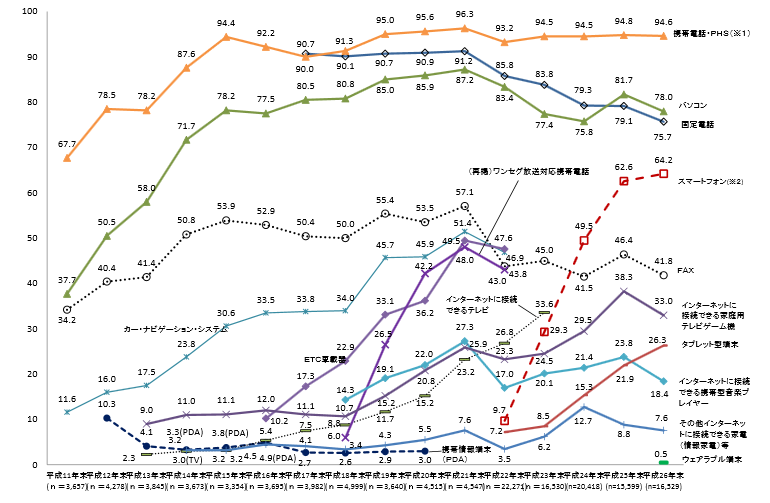
\includegraphics[width=16cm]{fig/n4301010.png}
\end{center}
\caption{情報通信端末の世帯保有数の推移(出典:総務省「平成25年度版 情報通信白書のポイント」)}
\end{figure}

また, スマートフォン, タブレット型端末は, それらが登場する以前に普及していたフィーチャーフォンやPHSとは圧倒的な機能差があり, 非常に多機能なデバイスである.
その多機能性を利用したシステムも数多く開発されており, GPSを利用したナビゲーションシステムや複数端末との通信を利用したソーシャルゲームなど, スマートデバイス普及以前では実現が難しかった様々なシステムが実用化され, 多くのユーザに利用されている.

本研究では, スマートフォン・タブレット型端末のポータビリティの高さとそれらの多機能性に着目し, 「ポータブルデバイスを入力とする情報収集アプリケーションの開発, および収集した情報を解析するWebアプリケーションの開発」を行い, スマートデバイスが収集する情報の正確性, データ解析の速度を調査する.
また, それらを連携させたシステムを試験し, 集積・解析ツールとして利用可能であるかを判定することを目的とする.

ポータビリティに特化しているスマートデバイスが収集し得る情報郡を集積し, それらを解析することによって, 「人々の動きの流れ」や「特定の地域で活動する時間帯」, 「どのような事物に興味を示すのか」など, 多種類の有用な市場情報を獲得することが可能となる.
獲得した情報を適切に利用することで, 市場における現状況の改善や新しい需要の創出等による経済的発展が期待できる.

スマートデバイスで収集可能な多数の情報の中から, 今回は“デバイスで撮影した写真データに記されている文字列”を対象とした情報収集, および収集データの解析を行う.
“画像データ内の文字列”を収集対象としたのは, 「沖縄県が全国有数の観光地である」こと, 「観光客が有名観光地の名称が入った場所で撮影を行う」こと, 「観光客がどの時間帯にどの観光地へ訪れるのかを解析したデータは, 県経済における観光収入の比率が大きい沖縄県において非常に有用な情報となる」ことが主な理由である.

\section{スマートデバイス}
2010年以降から普及しているスマートデバイスであるが, 現在, それらに搭載されている代表的なオペレーティングシステムとして, iOS, Androidが挙げられる.
さらに, タブレット型パーソナルコンピュータの開発, 販売競争も激化しており, 容易に持ち運びが可能なパソコンとしてMicrosoft Windows 10が普及し始めている.

表1.1に, 2013年から2015年にかけての, スマートデバイス用OSの市場占有率[2]のうち, iOS/Android/Windowsの推移を示す.

\begin{table}[htb]
\begin{center}
\begin{tabular}{|l|p{3cm}|p{3cm}|p{3cm}|} \hline
年月 & iOS(\%) & Android(\%) & Windows(\%) \\ \hline \hline
2013年1-3月 & 58.90 & 25.00 & 1.29 \\ \hline
2013年4-6月 & 58.70 & 25.05 & 1.22 \\ \hline
2013年7-9月 & 55.53 & 27.68 & 1.01 \\ \hline
2013年10-12月 & 54.91 & 33.39 & 0.57 \\ \hline
2014年1-3月 & 53.54 & 35.84 & 0.57 \\ \hline
2014年4-6月 & 48.32 & 41.06 & 1.65 \\ \hline
2014年7-9月 & 45.48 & 44.14 & 2.53 \\ \hline
2014年10-12月 & 43.99 & 46.03 & 2.27 \\ \hline
2015年1-3月 & 42.37 & 47.30 & 2.49 \\ \hline
2015年4-6月 & 39.49 & 51.74 & 2.26 \\ \hline
2015年7-9月 & 40.22 & 52.34 & 2.53 \\ \hline
2015年10-12月 & 36.86 & 55.68 & 2.87 \\ \hline
\end{tabular}
\caption{スマートデバイスのオペレーティングシステムの市場占有率の推移}
\end{center}
\end{table}

\subsection{iOS}
iOSとは, Apple Inc.が開発およびリリースしている, iPhone/iPod touch/iPad/iPad mini/Apple TVのオペレーティングシステムである.

2007年6月に発売された初代iPhoneと同時に提供され, 現在でも開発, 提供されている.(表1.2参照.)

\begin{table}[htb]
\begin{center}
\begin{tabular}{|l|l|p{10cm}|} \hline
バージョン & リリース年月 & 対応デバイス \\ \hline \hline
iPhone OS 1.0 & 2007年6月 & iPhone \\ \hline
iPhone OS 1.1 & 2007年9月 & iPhone, iPod touch \\ \hline
iPhone OS 2.0 & 2008年7月 & iPhone/3G, iPod touch \\ \hline
iPhone OS 2.1 & 2008年9月 & iPhone/3G, iPod touch \\ \hline
iPhone OS 2.2 & 2008年11月 & iPhone/3G, iPod touch \\ \hline
iPhone OS 3.0 & 2009年6月 & iPhone/3G/3GS, iPod touch \\ \hline
iPhone OS 3.1 & 2009年9月 & iPhone 3G/3GS, iPod touch \\ \hline
iPhone OS 3.2 & 2010年4月 & iPad \\ \hline
iOS 4.0 & 2010年6月 & iPhone 3GS/4, iPod touch, Apple TV \\ \hline
iOS 4.1 & 2010年9月 & iPhone 3GS/4, iPod touch, Apple TV \\ \hline
iOS 4.2.1 & 2010年11月 & iPhone 3GS/4, iPod touch, iPad/iPad 2, Apple TV \\ \hline
iOS 4.3 & 2011年3月 & iPhone 3GS/4, iPod touch, iPad/iPad 2, Apple TV \\ \hline
iOS 5.0 & 2011年10月 & iPhone 3GS/4/4S, iPod touch, iPad 2, Apple TV \\ \hline
iOS 5.1 & 2012年3月 & iPhone 3GS/4/4S, iPod touch, iPad/iPad 2, Apple TV \\ \hline
iOS 6.0 & 2012年9月 & iPhone 4/4S/5, iPod touch, iPad/Mini, Apple TV \\ \hline
iOS 6.1 & 2013年1月 & iPhone 4/4S/5, iPod touch, iPad/Mini, Apple TV \\ \hline
iOS 7.0 & 2013年9月 & iPhone 4S/5/5C/5S, iPod touch, iPad/Air/Mini/Mini 2, Apple TV \\ \hline
iOS 7.1 & 2014年3月 & iPhone 4S/5/5C/5S, iPod touch, iPad/Air/Mini/Mini 2, Apple TV \\ \hline
iOS 8.0 & 2014年9月 & iPhone 5/5C/5S/6/6 Plus, iPad/Air/Mini/Mini 2, Apple TV \\ \hline
iOS 8.1 & 2014年10月 & iPhone 5/5C/5S/6/6 Plus, iPad/Air 2/Mini/Mini 2/Mini 3, Apple TV \\ \hline
iOS 8.2 & 2015年3月 & iPhone 5/5C/5S/6/6 Plus, iPad/Air 2/Mini/Mini 2/Mini 3, Apple TV \\ \hline
iOS 8.3 & 2015年4月 & iPhone 5/5C/5S/6/6 Plus, iPad/Air 2/Mini/Mini 2/Mini 3, Apple TV \\ \hline
iOS 8.4 & 2015年6月 & iPhone 5/5C/5S/6/6 Plus, iPod touch, iPad/Air 2/Mini/Mini 2/Mini 3, Apple TV \\ \hline
iOS 9.0 & 2015年9月 & iPhone 5/5C/5S/6/6 Plus/6S/6S Plus, iPod touch, iPad/Air 2/Mini 2/Mini 3/Mini 4, Apple TV \\ \hline
iOS 9.1 & 2015年10月 & iPhone 5/5C/5S/6/6 Plus/6S/6S Plus, iPod touch, iPad/Air 2/Mini 2/Mini 3/Mini 4/Pro, Apple TV \\ \hline
iOS 9.2 & 2015年12月 & iPhone 5/5C/5S/6/6 Plus/6S/6S Plus, iPod touch, iPad/Air 2/Mini 2/Mini 3/Mini 4/Pro, Apple TV \\ \hline
\end{tabular}
\caption{iOSのメジャーバージョンと対応デバイスの変移}
\end{center}
\end{table}

iOSの最大の特徴は, Max OS Xと連携が取れる点である.s
iPhoneで撮影した画像や動画をMacに送信し編集する, iPhoneにかかってきた電話をMacで受ける, HandoffでMacで編集していた書類をiOSデバイスで編集するなど, iOSとMac OS Xの高い連携度によって, デバイスに依らない、柔軟性に富んだ作業を実施することが可能となっている.

\subsection{Android}
Androidは, Googleが開発およびリリースしている, Linuxカーネルをベースとした, スマートデバイス用オペレーティングシステムである.

2007年11月にAndroid 1.0が提供され, 現在でも開発, 提供されている.(表1.3参照.)

\begin{table}[htb]
\begin{center}
\begin{tabular}{|l|l|} \hline
バージョン & リリース年月 \\ \hline \hline
Android 1.0 & 2008年9月 \\ \hline
Android 1.1 & 2009年2月 \\ \hline
Android 1.5 Cupcake & 2009年4月 \\ \hline
Android 1.6 Donut & 2009年9月 \\ \hline
Android 2.0 Eclair & 2009年10月 \\ \hline
Android 2.1 Eclair & 2010年1月 \\ \hline
Android 2.2 Froyo & 2010年5月 \\ \hline
Android 2.3 Gingerbread & 2010年12月 \\ \hline
Android 3.0 Honeycomb & 2011年2月 \\ \hline
Android 3.1 Honeycomb & 2011年5月 \\ \hline
Android 3.2 Honeycomb & 2011年7月 \\ \hline
Android 4.0 Ice Cream Sandwich & 2011年10月 \\ \hline
Android 4.1 Jelly Bean & 2012年7月 \\ \hline
Android 4.2 Jelly Bean & 2012年11月 \\ \hline
Android 4.3 Jelly Bean & 2013年6月 \\ \hline
Android 4.4 KitKat & 2013年10月 \\ \hline
Android 5.0 Lollipop & 2014年11月 \\ \hline
Android 5.1 Lollipop & 2015年3月 \\ \hline
Android 6.0 Marchmallow & 2015年10月 \\ \hline
\end{tabular}
\caption{Androidのメジャーバージョンとリリース年月の一覧}
\end{center}
\end{table}

Androidは, Android SDKに対応しているスマートデバイスならば, どれでもそのOSとして無償で利用することが可能である.
また, 他のスマートデバイス向けオペレーティングシステムよりも, ミドルウェアやアプリケーションを作成する際の環境を構築することが容易である.
その高い自由性と対応性により, 2016年現在で最も利用されているスマートデバイス用オペレーティングシステムである.

\subsection{Microsoft Windows 10}
Microsoft Windows 10とは, Microsoft Corporationが開発およびリリースしている, Windowsシリーズに属するオペレーティングシステムである.

1985年11月にWindows 1.0が発表され, 現在でも開発, 提供されている.(表1.4参照.)

Windowsシリーズは, デスクトップ用オペレーティングシステムとしては, 2015年7月時点で約90\%のシェアを誇り, 現在最も利用されているデスクトップ用オペレーティングシステムである.

Windows 8以降は, タブレット型スマートデバイスでも利用することが可能となっており, 持ち運びの便利なタブレット型デバイスにWindows OSを搭載し利用するパソコンユーザも少なくない.

\begin{table}[htb]
\begin{center}
\begin{tabular}{|l|l|l|p{5.5cm}|} \hline
リリースネーム & バージョン & リリース年月 & 特徴 \\ \hline \hline
Windows 1.0 & 1.0 & 1985年11月 & MS-DOSコマンドを入力するのではなく, 画面上をマウスでクリックして動作させる \\ \hline
Windows 2.0 & 2.0 & 1987年12月 & コントロールパネル, キーボードショートカットの導入 \\ \hline
Windows 3.0 & 3.0 & 1990年5月 & プログラムマネージャ, ファイルマネージャ,の導入 \\ \hline
Windows 95 & 4.00 & 1995年8月 & スタートメニュー, タスクバー, ウィンドウの最小化/最大化/閉じるボタンの導入 \\ \hline
Windows 98 & 4.10 & 1998年6月 & コンシューマ向けに設計された初めてのバージョン \\ \hline
Windows 2000 & NT 5.0 & 2000年2月 & ファイル暗号化システム, Windows File Protectionの導入 \\ \hline
Windows ME & 4.90 & 2000年9月 & システム復元機能の導入 \\ \hline
Windows XP & NT 5.1 & 2001年10月 & 二列で構成されたスタートメニュー, タスクバーのタスク結合機能の導入 \\ \hline
Windows Vista & NT 6.0 & 2007年1月 & 透明なウィンドウなどの視覚効果の導入 \\ \hline
Windows 7 & NT 6.1 & 2009年10月 & サムネイルプレビュー, 最近開いたファイルをリスト表示するジャンプリストの導入 \\ \hline
Windows 8 & NT 6.2 & 2012年10月 & タッチスクリーンデバイスへの対応, スタートボタンを廃止し, スタートスクリーンを導入 \\ \hline
Windows 8.1 & NT 6.3 & 2013年10月 & スタートボタンの復活, 最大4つのアプリケーションを並べて使用できる機能の導入 \\ \hline
Windows 10 & NT 10.0 & 2015年7月 & 生体認証テクノロジーの導入 \\ \hline
\end{tabular}
\caption{Microsoft Windowsのメジャーバージョンとリリース年月の一覧}
\end{center}
\end{table}

\begin{figure}[htb]
\begin{center}
\begin{tabular}{c}

\begin{minipage}{0.5\hsize}
\begin{center}
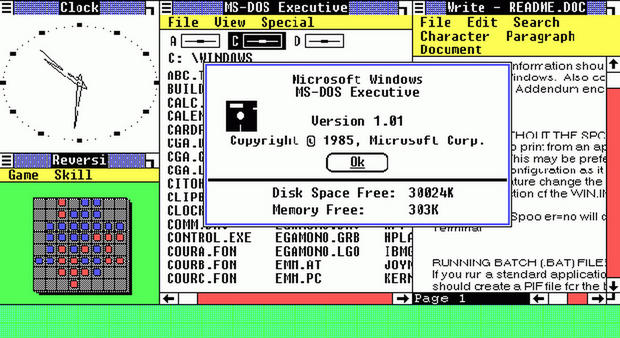
\includegraphics[width=7.5cm]{fig/windows1.jpg}
\caption{Windows 1.0のデスクトップ画面}

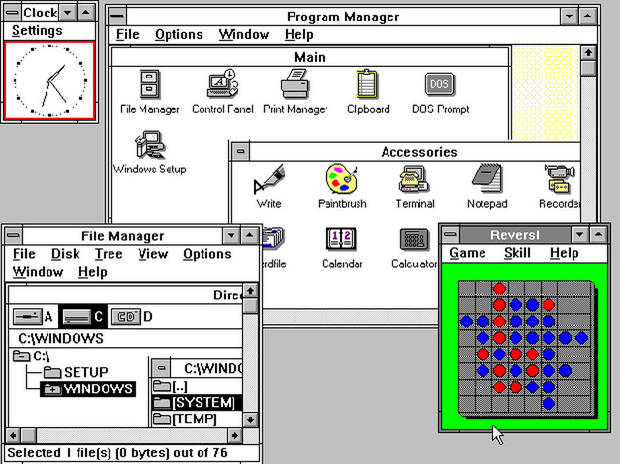
\includegraphics[width=7.5cm]{fig/windows3.jpg}
\caption{Windows 3.0のデスクトップ画面}

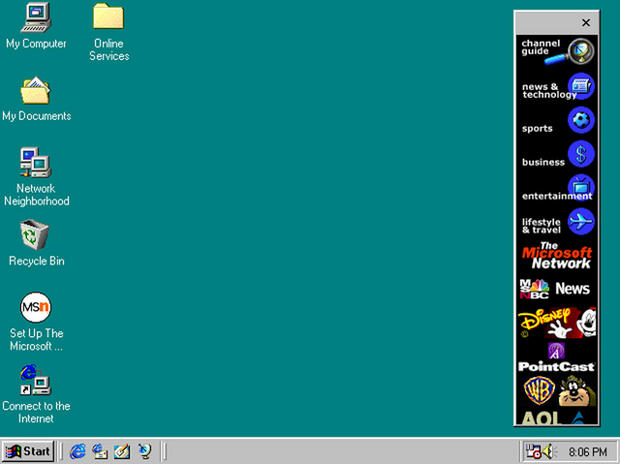
\includegraphics[width=7.5cm]{fig/windows98.jpg}
\caption{Windows 98のデスクトップ画面}
\end{center}
\end{minipage}

\begin{minipage}{0.5\hsize}
\begin{center}
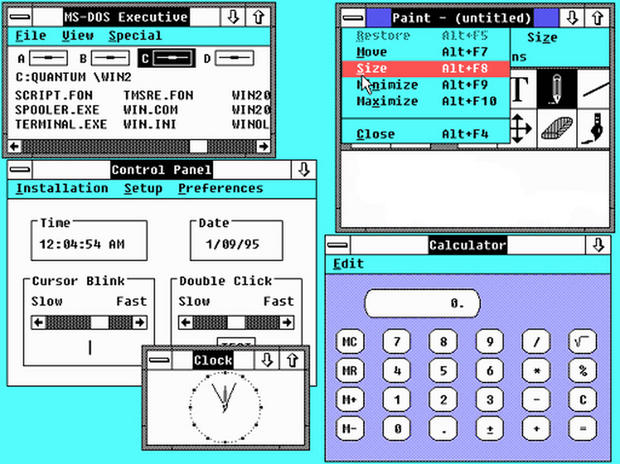
\includegraphics[width=7.5cm]{fig/windows2.jpg}
\caption{Windows 2.0のデスクトップ画面}

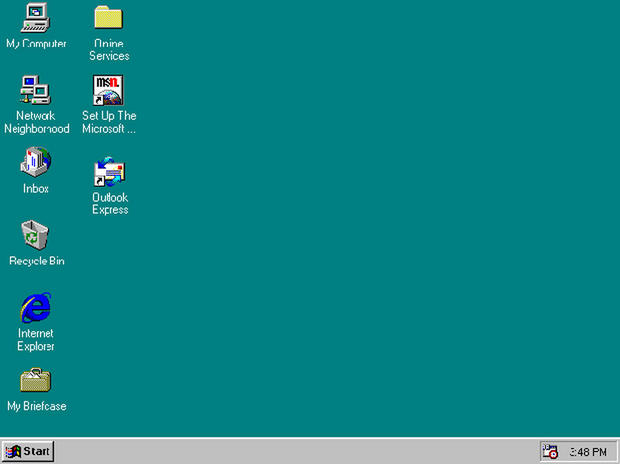
\includegraphics[width=7.5cm]{fig/windows95.jpg}
\caption{Windows 95のデスクトップ画面}

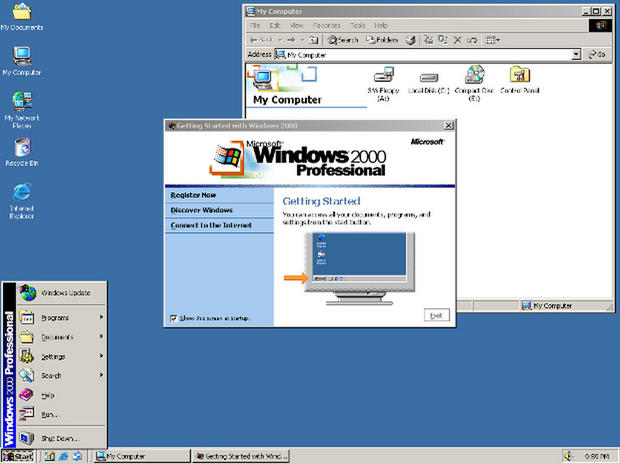
\includegraphics[width=7.5cm]{fig/windows2000.jpg}
\caption{Windows 2000のデスクトップ画面}
\end{center}
\end{minipage}

\end{tabular}
\end{center}
\end{figure}

\begin{figure}[htb]
\begin{center}
\begin{tabular}{c}

\begin{minipage}{0.5\hsize}
\begin{center}
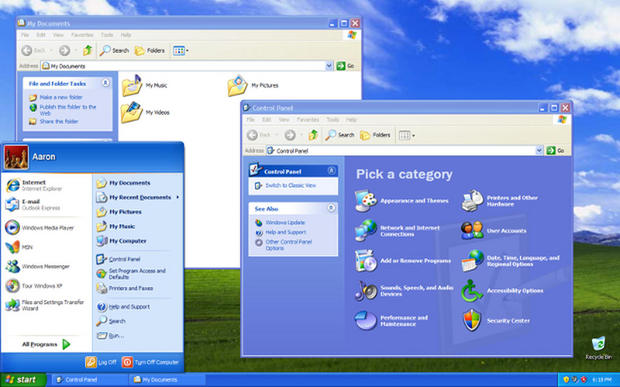
\includegraphics[width=7.5cm]{fig/windowsXP.jpg}
\caption{Windows XPのデスクトップ画面}

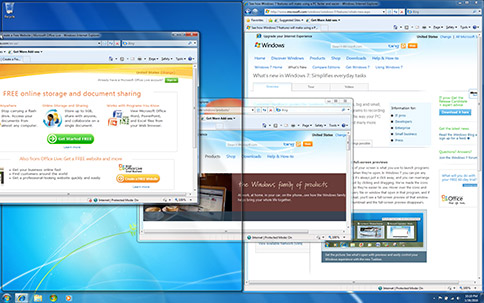
\includegraphics[width=7.5cm]{fig/windows7.jpg}
\caption{Windows 7のデスクトップ画面}

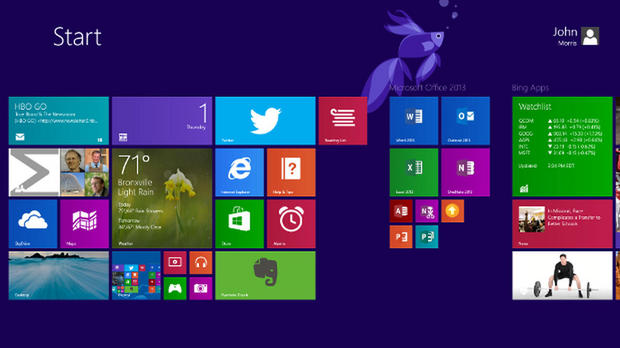
\includegraphics[width=7.5cm]{fig/windows8_1.jpg}
\caption{Windows 8.1のデスクトップ画面}
\end{center}
\end{minipage}

\begin{minipage}{0.5\hsize}
\begin{center}
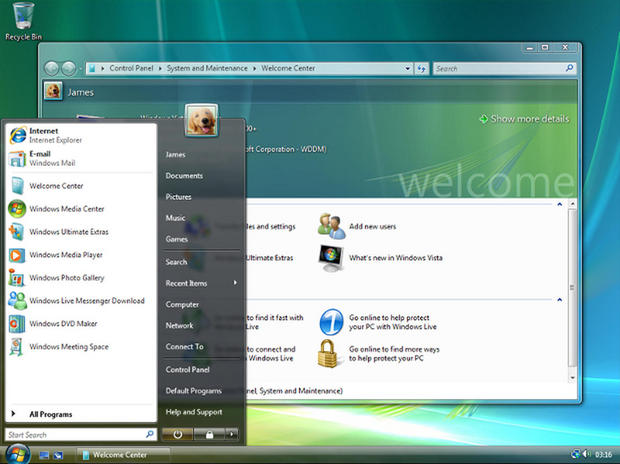
\includegraphics[width=7.5cm]{fig/windowsVista.jpg}
\caption{Windows Vistaのデスクトップ画面}

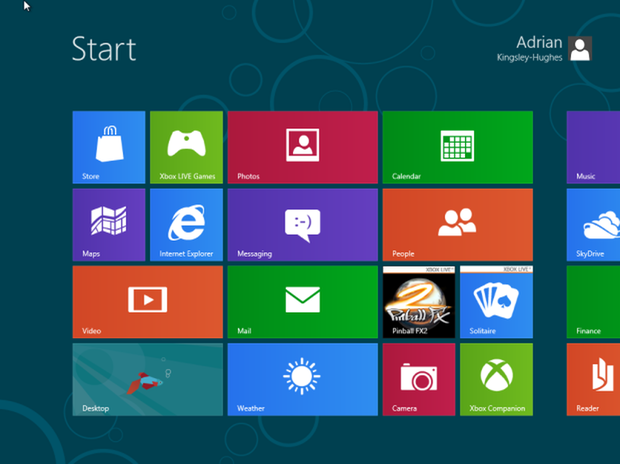
\includegraphics[width=7.5cm]{fig/windows8.png}
\caption{Windows 8のデスクトップ画面}

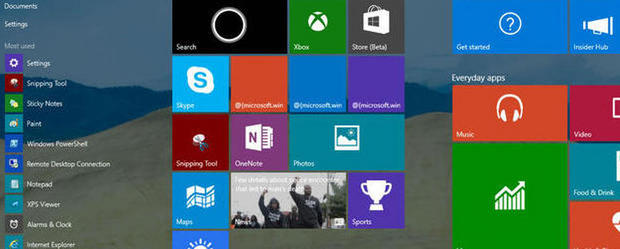
\includegraphics[width=7.5cm]{fig/windows10.jpg}
\caption{Windows 10のデスクトップ画面}
\end{center}
\end{minipage}

\end{tabular}
\end{center}
\end{figure}

\subsection{本研究で使用するスマートデバイス用オペレーティングシステム}
本研究では, 使用するスマートデバイス用オペレーティングシステムをiOSとする.

その理由として, 以下を挙げる.

\begin{itemize}
\item ポータビリティの高さ

iOSデバイスは, スマートデバイスでは現在2位の市場占有率を誇り, そのポータビリティはデータの回収に高い信頼性があると判断した.

\item 開発環境の構築の容易さ

琉球大学工学部情報工学科では, 講義にMacbookを使用しており, iOS/OS X用アプリケーションの開発ツールスイーツであるXcodeとObjective-Cのリファレンスなど, iOSデバイスのアプリケーションを作成するための環境を構築することが容易であるため.

また, 講義でiOSアプリケーションの開発言語であるObjective-Cを学んだことも, iOSデバイスを使用する要因の一つである.
\end{itemize}

\section{論文の構成}
本論文では, 第二章「技術概要」にて本研究にて使用したプログラミング言語やライブラリを解説する.

第三章「実験」では, どのようにしてiOSアプリケーションとWebアプリケーションが連携しているのかを示す.

第四章「本研究の利用例, 利用アイデア」では, 本研究をどのように活かせるのかを考察する.


\chapter{開発環境}
\label{chap:concept}

\section{iOSアプリケーション}
本研究では, Mac OS Xに搭載されている開発ツールスイートであるXcodeを用いてiOSアプリケーションを開発する.

\subsection{Objective-C}
Objective-Cとは, C言語をベースとして開発されたプログラミング言語である.

\begin{quotation}
\begin{screen}
“NEXTSTEP\footnote{NeXTコンピュータに搭載されたオブジェクト指向マルチタスクオペレーションシステム.}とMac OS X\footnote{Machintoshコンピュータに搭載されているオペレーティング・システム.}に標準付属されており, 現在は主にMac OS XとiOS上で動作するアプリケーションを開発する際に利用されている.
Objective-CはGCCによってコンパイル可能であるため, 基本的にはUNIX, Linix系OSや, GCCコンパイラを使用できる環境であればプログラムを動作させることが可能である.“

“C言語にSmalltalkをマクロ的拡張として施した言語であり, C言語により近い拡張を施されたC++と異なり, C言語とオブジェクト指向が混在した言語であると述べるほうが適切である.”

“if/for/whileなどの制御文や, int/char/floatなどのスカラー型, 関数記法, 宣言や代入といった基本的な文法はC言語に準拠しているが, オブジェクト指向はSmalltalkの概念を借用したものであり, その大きな特徴である「メッセージパッシングによるメソッド呼び出しを利用した, 記述力に優れたオブジェクトシステム」を継承している.”
\end{screen}
\end{quotation}
\begin{flushright}
(出典:\url{https://ja.wikipedia.org/wiki/Objective-C})
\end{flushright}

\begin{description}
\item (A) Objective-Cの特徴

Objective-Cによるオブジェクト指向開発環境[2]は, 以下の3要素から成り立つ.

\begin{description}
\item a) オブジェクト

\begin{quotation}
\begin{screen}
“オブジェクト指向言語を利用したプログラムは, オブジェクトと呼ばれる要素を中心に構成される.
オブジェクトとは, データと, そのデータを利用したりデータに作用する特定の関数による操作を関連付けたものをいう.
これらの操作はオブジェクトのメソッドと呼ばれる.
メソッドが作用するデータをインスタンス変数という.”

“よって, オブジェクトはインスタンス変数とメソッドを, 自己完結型のプログラミング単位にまとめたものと言い換えることができる.”

“Objective-Cでは, オブジェクトのインスタンス変数はオブジェクト内に存在し, 一般には, オブジェクトのメソッドによってのみ作用される.”

“他のメソッドがインスタンス変数に格納されているデータを得るには, アクセスしたいインスタンス変数を内包しているオブジェクトが, データを提供するメソッドを実装していなければならないが, インスタンス変数の有効範囲を指定することで, サブクラスや他のオブジェクトからインスタンス変数に直接アクセスすることも可能である.”
\end{screen}
\end{quotation}
\begin{flushright}
(出典:\url{https://developer.apple.com/jp/documentation/ObjC.pdf})
\end{flushright}

\item b) 開発ツールスイート

\begin{quotation}
\begin{screen}
“Objective-Cで開発を行うための開発ツールとして代表的なものに, Xcodeが挙げられる.”

“Xcodeは, Apple Inc.が開発, 配布している, Mac/iPhone/iPad/Apple Watch向けアプリケーション開発用のデベロッパツールセットである.”

“ユーザインターフェースのデザイン, コーディング, テスト, デバッグ, Apple Storeへの提出を行えることによる, スムーズなアプリケーション開発を実現している.”

“また, Xcodeには, Xcode IDE(統合開発環境:Integrated Development Environment), SwiftおよびObjective-Cのプログラミング言語向けコンパイラ, Instruments分析ツール, iOS Simukator, 最新のiOS/OS X向けSDKなどの機能も用意されている.”
\end{screen}
\end{quotation}
\begin{flushright}
(出典:\url{https://developer.apple.com/jp/documentation/ObjC.pdf})
\end{flushright}

\item c) ランタイム環境

\begin{quotation}
\begin{screen}
“Objective-Cでは, 可能な限り多くの決定が実行時に行われる.
オブジェクトの作成やどのメソッドを呼び出すかの決定などの動作は動的に実行されるため, Objective-Cでは, コンパイラだけでなく, コンパイルしたコードを実行するランタイムシステムも必要となる.

“ランタイムシステムは, Objective-Cにとって, 一種のオペレーティングシステムとして動作し, 言語を機能させる.”
\end{screen}
\end{quotation}
\begin{flushright}
(出典:\url{https://developer.apple.com/jp/documentation/ObjC.pdf})
\end{flushright}

\end{description}

\item (B) Objective-C 2.0

Apple Inc.はMac OS X v10.5 Leopardにおいて, 言語仕様を変更したObjective-C 2.0を発表した.
Objective-C 2.0では, ガベージコレクションとプロパティの導入, foreach文の採用, 実装オプションのプロトコル定義の増加, 非公開プライベートメソッドが実装可能, ランタイム構造の変更などが行われた.
\end{description}

\subsection{OpenCV}
OpenCV(Open Source Computer Vision Library)とは, Intel Corporationが開発, 公開しているオープンソースのコンピュータビジョン用ライブラリである.

\begin{quotation}
\begin{screen}
“画像処理, 画像解析, 機械学習の機能を持つC/C++, Java, Python, MATLAB用ライブラリで, プラットフォームとしてUnix/Linux系OS, Windows, Android, iOSなどをサポートしている.
BSDライセンスで配布されているため, 学術目的のみでなく, 商用目的でも利用することが可能である.”
\end{screen}
\end{quotation}
\begin{flushright}
(出典:\url{https://ja.wikipedia.org/wiki/OpenCV})
\end{flushright}

1999年に開発プロジェクトが開始され, 2000年のアルファ版公開を皮切りに, 2001年から2005年にかけて, 5つのベータ版が公開されている.
正式版のリリース後, 2016年1月現在まで開発, 公開されている(表2.1).

\begin{table}[tb]
\begin{center}
\begin{tabular}{|l|l|l|} \hline
バージョン & リリース年月 & 公式サポート言語 \\ \hline \hline
1.0 & 2006年10月 & C言語 \\ \hline
2.0 & 2009年10月 & C言語, C++ \\ \hline
2.1 & 2010年4月 & C言語, C++ \\ \hline
2.2 & 2010年12月 & C言語, C++, Python \\ \hline
2.3 & 2011年7月 & C言語, C++, Python \\ \hline
2.4 & 2012年5月 & C言語, C++, Python \\ \hline
2.4.1 & 2012年6月 & C言語, C++, Python \\ \hline
2.4.2 & 2012年7月 & C言語, C++, Python \\ \hline
2.4.3 & 2012年11月 & C言語, C++, Python \\ \hline
2.4.4 & 2013年3月 & C言語, C++, Python, Java \\ \hline
2.4.5 & 2013年4月 & C言語, C++, Python, Java \\ \hline
2.4.6 & 2013年7月 & C言語, C++, Python, Java \\ \hline
2.4.7 & 2013年11月 & C言語, C++, Python, Java \\ \hline
2.4.8 & 2013年12月 & C言語, C++, Python, Java \\ \hline
2.4.9 & 2014年4月 & C言語, C++, Python, Java \\ \hline
2.4.10 & 2014年10月 & C言語, C++, Python, Java \\ \hline
2.4.11 & 2015年2月 & C言語, C++, Python, Java \\ \hline
3.0 & 2015年6月 & C++, Python, Java(3.0以降, C言語はメンテナンス対象外) \\ \hline
3.1 & 2015年12月 & C++, Python, Java \\ \hline
\end{tabular}
\caption{OpenCVのバージョンとリリース年月, 公式サポート言語の一覧}
\end{center}
\end{table}

最新バージョンであるOpenCV 3.x系列では, C言語関数形式のインターフェイスがメンテナンス対象外とされ, C++ APIを利用することが推奨されている.

\begin{description}
\item (A) OpenCVの機能

OpenCVに実装されている機能としては, フィルター処理, 変形処理, 構造解析と形状ディスクリプタ, 物体検出, モーション解析と物体追跡, 領域分割, カメラキャリブレーション, 特徴点検出, 機械学習がある[4].

\begin{description}
\item a) フィルター処理

OpenCVにおけるフィルタリングは, 二次元配列であるMat型で定義された二次元画像に対して処理を実行する.
画像の平滑化や収縮/膨張などの処理を行うことで, 画像のぼかしやノイズキャンセリングを施す.

\item b) 変形処理

二次元画像の幾何学変換を行い, 変形画像をマッピングする.
この処理を施す際は画像の内容そのものは変更されず, ピクセルの座標移動のみを行う..

\item c) 構造解析と形状ディスクリプタ

二次元画像内に描かれている, あるいは含まれている特定の形状を検出する.
画像内の特定の形状のみを認識したい場合等で利用する.

\item d) 物体検出

予め設定しているテンプレートと二次元画像とを比較し, テンプレートとマッチングする物体を検出する.
顔認識や指紋認識など, 生体認証等で利用する.

\item e) モーション解析と物体追跡

動画内で動いている物体の動きを認識する, あるいは動体を追跡する.
モーション検知や動体検知等で利用する.

\item f) 領域分割

二次元画像を形状や色などの特徴を用いて, 複数の領域に分割する.
特定の領域のみで画像処理を施す場合や, 特定の領域のみを抜き出す場合等で利用する.

\item g) カメラキャリブレーション

カメラ固有の内部パラメータと, ワールド座標系における位置や姿勢を意味する外部パラメータを求める.
カメラで撮影した二次元画像の歪みを補正する場合等で利用する.

\item h) 特徴点検出

二次元画像における特徴点を検出する.
特徴点を検出してパターンマッチングを行う場合等で利用する.

\item i) 機械学習

OpenCVでは, ニューラルネットワークを用いた機械学習を実装することが可能である.
二次元画像を教師データとして入力し, 形状や物体の認識率を向上させる場合等で利用する.
\end{description}

\end{description}

\subsection{Tesseract-OCR}
Tesseract-OCRとは, ヒューレット・パッカード研究所とヒューレット・パッカード社が開発し, 現在はGoogleが開発, 配布している, 光学文字認識用のオープンソースライブラリである.

ライブラリの大半はC言語で書かれており, 一部はC++で書かれている.
そのため, C言語コンパイラがインストールされているならば, 様々な環境で動作させる事ができる.

Tesseract-OCRは2016年1月現在, 64の言語に対応している(表2.2).

\begin{table}[tb]
\begin{center}
\begin{tabular}{|p{3.5cm}|p{3.5cm}|p{3.5cm}|p{3.5cm}|} \hline
英語 & ウクライナ語 & トルコ語 & タイ語 \\ \hline
タガログ語 & テルグ語 & タミル語 & スウェーデン語 \\ \hline
スワヒリ語 & セルビア語 & アルバニア語 & スペイン古語 \\ \hline
スペイン語 & スロベニア語 & スロバキア語 & ローマ語 \\ \hline
ポルトガル語 & ポーランド語 & ノルウェー語 & オランダ語 \\ \hline
マレー語 & マルタ語 & マケドニア語 & マラヤーラム語 \\ \hline
リトアニア語 & ラトビア語 & 韓国語 & カナダ語 \\ \hline
イタリア古語 & イタリア語 & アイスランド語 & インドネシア語 \\ \hline
チェロキー語 & ハンガリー語 & クロアチア語 & ヒンディー語 \\ \hline
ヘブライ語 & ガルシア語 & 中世フランス語 & フランス語 \\ \hline
フランク語 & フィン語 & バスク語 & エストニア語 \\ \hline
エスペラント語 & 中世英語 & グリーク語 & ドイツ語 \\ \hline
デンマーク語 & チェコ語 & カタロニア語 & ブルガリア語 \\ \hline
ブルガリア語 & ベンガル語 & ベラルーシ語 & アゼルバイジャン語 \\ \hline
アラビア語 & アフリカ語 & 日本語 & 中国語(簡体字) \\ \hline
中国語(繁体字) & ロシア語 & ベトナム語 & 数学記号 \\ \hline
\end{tabular}
\caption{Tesseract-OCRにて認識可能な言語一覧}
\end{center}
\end{table}

Tesseract-OCRはニューロンネットワークによる機械学習を実装しており, 上記の言語のデータを教師データとして与えることにより, 文字の認識率を向上させることが可能である.

\section{Webアプリケーション}
本研究では, Rubyで開発されたWebアプリケーションフレームワークで高いシェアを誇るRuby on Railsを用いてWebアプリケーションを開発する.

Webアプリケーションの開発環境は, 琉球大学工学部情報工学科が管理, 提供しているVPSサーバに構築した.

\section{VPSサーバの環境}
\subsection{CentOS}
CentOSとは, The CentOS Projectがオープンソースライセンスで開発, 配布しているLinixディストリビューションである.

\begin{quotation}
\begin{screen}
“CentOSという名称は「コミュニティベースで開発された, 有償版に匹敵するオペレーティングシステム(Community ENTerprise Operating System)」が由来となっている.”

“2004年5月のリリースから, RHELの最新版が公開される度に, その後を追うようにしてメジャーアップデートを重ね, 2016年1月現在まで開発, 配布されている.”

“Red Hat Enterprise Linux(RHEL)\footnote{Red Hat社が開発, 販売している業務向けLinuxディストリビューション.}の完全互換を目指して開発され, Red Hat社がオープンソースにて公開しているRHELのソースコードを基に, Red Hat社の商標や商用パッケージを除去し, リビルドしたものがCentOSである.
このことから, CentOSは一般に「RHELクローン」\footnote{RHELを基としたLinuxディストリビューション全般を含んだ呼称であるため, White Box Enterprise LinuxやScientific LinuxもRHELクローンに含まれる.}と呼称されることもある.”
\end{screen}
\end{quotation}
\begin{flushright}
(出典:\url{https://ja.wikipedia.org/wiki/CentOS})
\end{flushright}

Linuxをベースとしたオペレーティングシステムであること, GNUライセンスによる配布による低コストでの導入の容易さから, 主に中小規模のプロジェクトにて採用されることが多い.

\subsection{Ruby on Rails}
Ruby on Railsとは, Rails Core Teamが開発, 提供しているオープンソースのWebアプリケーションフレームワークである.

オブジェクト指向スクリプト言語であるRubyにて記述されており, オブジェクト指向を強く意識したフレームワークとなっている.

2004年10月に正式版がリリースされてから, 2016年1月現在まで開発, 公開されている.

\begin{comment}
\begin{table}[tb]
\begin{center}
\begin{tabular}{|l|l|} \hline
バージョン & リリース年月 \\ \hline \hline
0.8.0 & 2004年10月 \\ \hline
0.9.0 & 2004年12月 \\ \hline
0.10.0 & 2005年2月 \\ \hline
0.11.0 & 2005年3月 \\ \hline
0.12.0 & 2005年4月 \\ \hline
0.13.0 & 2005年7月 \\ \hline
0.14.1 & 2005年10月 \\ \hline
1.0.0 & 2005年12月 \\ \hline
1.1.0 & 2006年3月 \\ \hline
1.2.0 & 2007年1月 \\ \hline
2.0.0 & 2007年12月 \\ \hline
2.1.0 & 2008年5月 \\ \hline
2.2.2 & 2009年11月 \\ \hline
2.3.2 & 2009年5月 \\ \hline
3.0.0 & 2010年8月 \\ \hline
3.1.0 & 2011年8月 \\ \hline
3.2.0 & 2012年1月 \\ \hline
4.0.0 & 2013年6月 \\ \hline
4.1.0 & 2014年4月 \\ \hline
4.2.0 & 2014年12月 \\ \hline
4.2.5 & 2015年11月 \\ \hline
\end{tabular}
\caption{Ruby on Railsのメジャーバージョンとリリース年月の一覧}
\end{center}
\end{table}
\end{comment}

\begin{description}
\item (A)Webアプリケーションフレームワーク

\begin{quotation}
\begin{screen}
“Webアプリケーションフレームワークとは, 動的なウェブサイト, Webアプリケーション, Webサービスの開発をサポートするために設計されたアプリケーションフレームワークである.”

“アプリケーションフレームワークとは, 特定のオペレーティングシステムのためのアプリケーションの標準構造を実装するのに使われるクラスやライブラリの集合である.”
\end{screen}
\end{quotation}
\begin{flushright}
(出典:\url{https://ja.wikipedia.org/wiki/Ruby_on_Rails})
\end{flushright}

つまり, 端的にWebアプリケーションフレームワークを言い換えると, Webアプリケーションを開発する際に必要なクラスやライブラリを提供する, Webアプリケーションの土台となるものとなる.

HTMLやPHP等の, Webページ/アプリケーションを開発するための言語を扱うことに長けた専門家が, それらの言語を用いて一から開発したアプリケーションと同等のものが, Webアプリケーションフレームワークを用いることで, 初心者でも開発することが可能となる[5].

\item (B) Ruby on Railsの特徴

Ruby on Railsの特徴は, その開発理念である“同じことを繰り返さない(DRY:Don't Repeat Yourself)”と'“設定より規約(CoC:Convention over Configuration)”の順守による, 実アプリケーションの開発が他のフレームワークよりも少ないコードで簡単に行える点である.

“同じことを繰り返さない”とは, 「定義などの作業は一度のみ行う」, 「重複するコードを記述しない」という意味である.

“設定より規約”とは, 「慎重に設定された規約に従うことで, 設定を不要にする, あるいは軽減する」という意味である.

これらの基本理念により, Ruby on Railsでは, コンソール上でコマンドを入力することで, 命名規則に従った複数の関連付けられたファイルが生成されるため, ファイル構成の把握が非常に簡易である.

このRuby on Railsのコンセプトに影響を受けたフレームワークとして, PHPのCakePHPやSymfony, PerlのCatalyst, JavaのGrailsといったものが挙げられる.

\item (C) Ruby on RailsにおけるMVCアーキテクチャ

Ruby on RailsはMVC(Model View Controller)アーキテクチャを採用している.

\begin{quotation}
\begin{screen}
“MVCアーキテクチャとは, アプリケーションの構造をModel/View/Controllerの3つの要素に分割し, アプリケーションの内部データを利用者が直接参照することがないようにしたものである(図2.1).”
\end{screen}
\end{quotation}
\begin{flushright}
(出展:\url{https://ja.wikipedia.org/wiki/Model_View_Controller})
\end{flushright}

\begin{figure}
\begin{center}
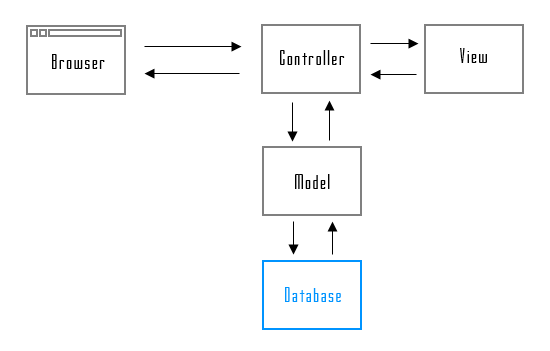
\includegraphics[width=13cm]{fig/mvc.png}
\caption{MVCアーキテクチャの簡略図}
\end{center}
\begin{flushright}
(出展:\url{http://www.rubylife.jp/rails/ini/index7.html})
\end{flushright}
\end{figure}

\begin{itemize}
\item Model

\begin{quotation}
\begin{screen}
“アプリケーションが扱う領域のデータと手続きを表現した要素.
データの変更をビューに通知するのもModelの役割である.”
\end{screen}
\end{quotation}
\begin{flushright}
(出展:\url{https://ja.wikipedia.org/wiki/Model_View_Controller})
\end{flushright}

\begin{quotation}
\begin{screen}
“Ruby on RailsにおけるModelは, 使用しているデータベースのテーブルごとにModelが用意されている.
利用者からのリクエストで呼びだされたアクションは, Modelを介してデータベースとのやり取りを行い, データの取得や新しいデータの格納を行う(図2.2).”
\end{screen}
\end{quotation}
\begin{flushright}
(出典:\url{http://www.rubylife.jp/rails/ini/index7.html})
\end{flushright}

\begin{figure}
\begin{center}
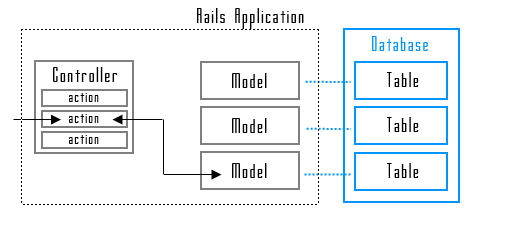
\includegraphics[width=13cm]{fig/model.png}
\caption{Modelの動作簡略図}
\begin{flushright}
(\url{http://www.rubylife.jp/rails/ini/index7.html})
\end{flushright}
\end{center}
\end{figure}

\item View

\begin{quotation}
\begin{screen}
“Modelのデータを取り出し, ユーザが見るのに適した形となるHTML文書を作成する要素.
すなわち, データをブラウザへ出力するための雛形を作成するのが役割である.”
\end{screen}
\end{quotation}
\begin{flushright}
(出典:\url{https://ja.wikipedia.org/wiki/Model_View_Controller})
\end{flushright}

\begin{quotation}
\begin{screen}
“Ruby on RailsにおけるViewは, アプリケーション内に複数用意されている.
Viewの1つ1つが与えられたデータから生成されたHTML文書となっている.
アクションに対応するViewが1つ用意されており, アクションが実行されると, 紐付けされたViewが呼び出されて利用者へ返すWebページを作成する(図2.3).”
\end{screen}
\end{quotation}
\begin{flushright}
(出典:\url{http://www.rubylife.jp/rails/ini/index7.html})
\end{flushright}

\begin{figure}
\begin{center}
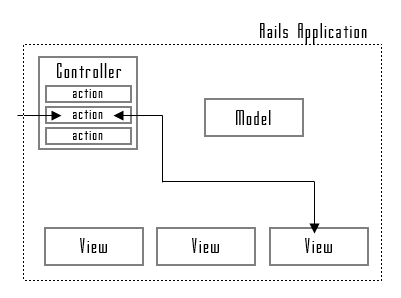
\includegraphics[width=13cm]{fig/view.png}
\caption{Viewの動作簡略図}
\end{center}
\begin{flushright}
(出典:\url{http://www.rubylife.jp/rails/ini/index7.html})
\end{flushright}
\end{figure}

\item Controller

\begin{quotation}
\begin{screen}
“ユーザからの入力をModelへのメッセージに変換し, 伝える要素である.
すなわち, UIからの入力を担当する.”
\end{screen}
\end{quotation}
\begin{flushright}
(出典:\url{https://ja.wikipedia.org/wiki/Model_View_Controller})
\end{flushright}

\begin{quotation}
\begin{screen}
“Ruby on RailsにおけるControllerは, アプリケーション内に複数用意されている.
また, 各Controllerの中には複数のアクションが定義されており, URLとして届いた利用者のリクエストを分析し, どのControllerに含まれるどのアクションを実行すべきか判断するための「ルーティング」が行われる(図2.4).”
\end{screen}
\end{quotation}
\begin{flushright}
(出典:\url{http://www.rubylife.jp/rails/ini/index7.html})
\end{flushright}

\begin{figure}
\begin{center}
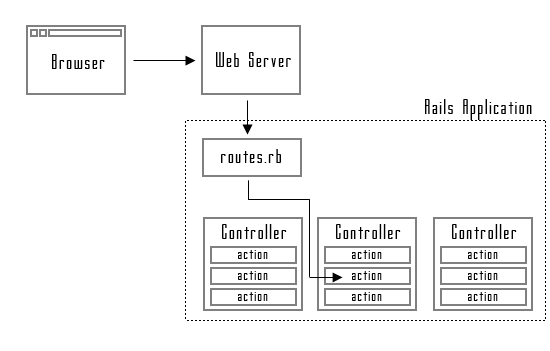
\includegraphics[width=13cm]{fig/route.png}
\caption{ルーティング}
\end{center}
\begin{flushright}
(\url{http://www.rubylife.jp/rails/ini/index7.html})
\end{flushright}
\end{figure}

\begin{quotation}
\begin{screen}
“ルーティングによって次に行われるべきアクションが決定した際, そのアクションに紐付けされたModelがデータベースとのやり取りを, Viewがユーザへ返すHTML文書を作成する.
返ってきたHTML文書をControllerがリクエストした利用者に見える形でブラウザに返す(図2.5).”
\end{screen}
\end{quotation}
\begin{flushright}
(出典:\url{http://www.rubylife.jp/rails/ini/index7.html})
\end{flushright}

\begin{figure}
\begin{center}
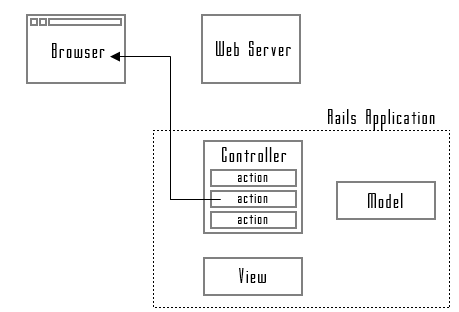
\includegraphics[width=13cm]{fig/controller.png}
\caption{Controllerの動作簡略図}
\end{center}
\begin{flushright}
(\url{http://www.rubylife.jp/rails/ini/index7.html})
\end{flushright}
\end{figure}

\end{itemize}

\end{description}

\subsection{PostgreSQL}
PostgreSQLとは, PostgreSQL Global Development Groupがオープンソースで開発, 配布している, オブジェクト関係データベース管理システム(ORDBMS:Objective Relational DataBase Management System)である.

1995年5月に正式版がリリースされてから, 2016年1月現在まで開発, 公開されている(表2.4).

\begin{comment}
\begin{table}[tb]
\begin{center}
\begin{tabular}{|l|l|} \hline
バージョン & リリース年月 \\ \hline \hline
0.01 & 1995年5月 \\ \hline
1.0 & 1995年9月 \\ \hline
6.0 & 1997年1月 \\ \hline
6.1 & 1997年6月 \\ \hline
6.2 & 1997年10月 \\ \hline
6.3 & 1998年3月 \\ \hline
6.4 & 1998年10月 \\ \hline
6.5 & 1999年6月 \\ \hline
7.0 & 2000年5月 \\ \hline
7.1 & 2001年4月 \\ \hline
7.2 & 2002年2月 \\ \hline
7.2 & 2002年11月 \\ \hline
7.4 & 2003年11月 \\ \hline
8.0 & 2005年1月 \\ \hline
8.1 & 2005年11月 \\ \hline
8.2 & 2006年12月 \\ \hline
8.3 & 2008年2月 \\ \hline
8.4 & 2009年7月 \\ \hline
9.0 & 2010年9月 \\ \hline
9.1 & 2011年9月 \\ \hline
9.2 & 2012年9月 \\ \hline
9.3 & 2013年9月 \\ \hline
9.4 & 2014年12月 \\ \hline
9.5 & 2016年1月 \\ \hline
\end{tabular}
\caption{PostgreSQLのメジャーバージョンとリリース年月の一覧}
\end{center}
\end{table}
\end{comment}

PostgreSQLは, オープンソースなリレーショナルデータベース管理システム(RDBMS)であるIngresから発展したプロジェクトである.

\begin{quotation}
\begin{screen}
“PostgreSQLという名は, 「Post-Ingres」, つまり「Ingresの後継であること」と, 「SQLデータベース操作構文を用いてデータベース操作が可能であること」が, その名の由来となっている.
Ingresの課題であった, 「ユーザが新たな定義域を既存の単純な定義域から定義できない」という実装の限界に対処することを目的として開発された.”

“データベースの操作にはSQLデータベース操作構文を利用しているが, PL/pgSQL, PL/PSM, スクリプト言語(PL/Perl, PL/php, PL/Python, PL/Ruby, PL/Tcl, PL/Lua), コンパイラ言語(C言語, PL/Java), 統計処理言語(PL/R)の関数を実行することも可能である.”
\end{screen}
\end{quotation}
\begin{flushright}
(出典:\url{https://ja.wikipedia.org/wiki/PostgreSQL})
\end{flushright}

\begin{description}
\item (A) リレーショナルデータベース(Relational DataBase)

\begin{quotation}
\begin{screen}
“リレーショナルデータベースとは, 一見のデータを複数の属性(カラム)の値(フィールド)の組(レコード)として表現し, 組を列挙することでデータを格納していく方式のデータベースのことである.
属性を列, 組を業とする表(テーブル)の形で表されることが多い.
複数のテーブルに含まれる同じカラムを関連付けることができ, 複雑なデータや大規模なデータを柔軟に取り扱うことができる.”
\end{screen}
\end{quotation}
\begin{flushright}
(出典:\url{http://e-words.jp/w/RDBMS.html})
\end{flushright}

データベースの構造では最も普及しており, 単にデータベースといった場合はリレーショナルデータベースであることが多い.

\item (B) Relational DataBase Management System

Relational DataBase Management System(RDBMS)とは, リレーショナルデータベースを管理するための専用ソフトウェアである.

\begin{quotation}
\begin{screen}
“ストレージ内に専用の管理領域を確保し, テーブルの作成や消去, 構造の修正, データの追加, 検索, 抽出, 修正, 削除等を行う.
データベース管理者や利用者が直接操作を行う他に, 外部のソフトウェアから接続を受け付け, ソフトウェアのプログラムから操作を行うことも可能である.
RDBMSへの照会や操作の指示には, SQLと呼ばれるデータベース操作言語が標準として広く利用されている.”

“RDBMSは, 不正なデータの記録を拒否するなどしてデータベースの整合性を保つ, 権限のない利用者による不正な読み出しや改ざん等からデータを保護する等の仕組みを持つ.
また, 関連する複数の処理を一体化して矛盾なく実行するトランザクション処理を行ったり, 障害に備えてデータベースのバックアップを行い, 破損時には過去のある時点の状態へと復旧したりといった機能を備えたものもある.”
\end{screen}
\end{quotation}
\begin{flushright}
(出典:\url{http://e-words.jp/w/RDBMS.html})
\end{flushright}

\end{description}

\subsection{Heroku}
Herokuとは, 2007年に創業された同名の企業が開発と運営を行っている, PaaS(Platform as a Service)である.

Herokuは自社の目的として, “技術者をビジネスの本質的な価値提供(アプリケーション開発)に集中させること”, “開発者の生産性を最大化すること”を掲げており, PaaSの提供だけでなく, 高頻度の機能追加やアドオンの提供を行っている.

PaaSとは, アプリケーションを実行するためのプラットフォームである.

“アプリケーションを実行するためのプラットフォーム”は, 「ハードウェア」, 「ネットワーク」, 「仮想化環境」, 「オペレーティングシステム」, 「データベース」, 「アプリケーションフレームワーク」で構成されている.

Webアプリケーションを自らの手で一から全て開発する場合,
\begin{enumerate}
\item サーバPCやルータ等のハードウェアを購入

\item それらをインターネットに接続し, かつプライベート空間を分離するためのファイアウォールを含むネットワークを構築

\item サーバの仮想化環境を整備

\item LinuxやWindowsサーバ等のオペレーティングシステムをインストール

\item OracleやMySQL, PostgreSQL等のデータベースをセットアップ

\item JavaやRuby, PHP等のアプリケーション実行環境をセットアップ
\end{enumerate}

という手順を踏んで, アプリケーションを公開するための環境を整えなければならない.

PaaSは, これらのプラットフォームの構築にかかる様々な作業を代行してくれるサービスである.
PaaSを利用することで, 最初に行わなければならない環境構築への労力を軽減し, また, プラットフォームの保守運用にかかる費用を削減することが可能となる.

Webアプリケーション開発の補助を行うサービスとして, 「IaaS(Infrastructure as a Service)」, 「SaaS(Software as a Service)」があり, そして全てを自ら管理する「オンプレミス」がある(図2.1).

\begin{figure}
\begin{center}
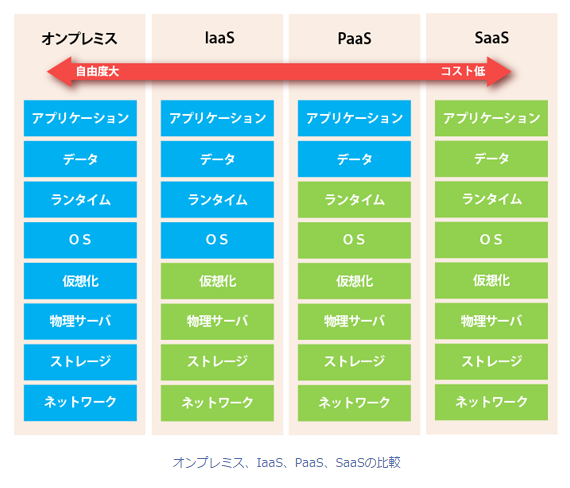
\includegraphics[width=16cm]{fig/paas.png}
\caption{オンプレミス, IaaS, PaaS, SaaSの比較}
\end{center}
\begin{flushright}
(\url{http://codezine.jp/article/detail/8051})
\end{flushright}
\end{figure}

\begin{itemize}
\item オンプレミス

プラットフォームの全てを自身で管理する.

「ハードウェア」, 「ネットワーク」, 「仮想化環境」, 「オペレーティングシステム」, 「データベース」, 「アプリケーションフレームワーク」を自身で選択できるため, 開発の自由度が高い.

しかし, 環境構築からアプリケーション公開までの労力は必然的に重たくなる.

\item IaaS

プラットフォームのうち, 「ハードウェア」, 「ネットワーク」, 「仮想化環境」までをサービス事業者が管理する.

「オペレーションシステム」, 「データベース」, 「アプリケーションフレームワーク」は自ら選択できるため, サービス利用者の慣れ親しんだ環境でのアプリケーション開発を行うことができる.

\item PaaS

プラットフォームの「ハードウェア」, 「ネットワーク」, 「仮想化環境」, 「オペレーティングシステム」, 「データベース」までをサービス事業者が管理する.

「アプリケーションフレームワーク」にて開発したアプリケーションをサービス会社のサーバにアップロードすることで, サービス事業者がランタイム(アプリケーションの実行)まで行う.

サービス利用者はアプリケーションの開発, 運用のみに注力すればよいが, 開発環境の自由度はIaaSよりも低い.

\item SaaS

プラットフォームの全てをサービス事業者が管理する.

管理コストは最も低いが, 開発環境の自由度も低い.

サービス事業者が提供するソフトウェアをインストールして利用する形態を採用しているため, サービス事業者によって開発可能なサービスが異なる可能性がある.
\end{itemize}

本研究では, Webアプリケーションをインターネット上で公開する際に利用するサービスとして, PaaSを提供しているHerokuを採用する.

その理由として,  「仮想環境の構築までは予め用意されている環境を使用し, Webアプリケーションは自ら選択したフレームワークで開発する」ためである.
また, 高頻度の機能追加や多種多様なアドオンの提供を実施しており, 開発環境を整えやすいのもHerokuを採用した理由の一つである.


\chapter{実装}
\label{chap:poordirection}

\section{システムの流れ}
本研究にて構築するシステムは, 主に「iOSアプリケーション」, 「Webアプリケーション」, 「データベース」の三要素にて成り立つ.(図3.1参照.)

\section{iOSアプリケーション}
iOSアプリケーションを作成するにあたり, 以下の言語とライブラリ, 統合開発環境を利用した.(表3.1参照.)

\begin{table}
\begin{center}
\begin{tabular}{|l|l|} \hline
Xcode &  \\ \hline
Objective-C 2.0 & \\ \hline
Tesseract-OCR & \\ \hline
OpenCV & \\ \hline
\end{tabular}
\end{center}
\caption{iOSアプリケーション作成時に利用した環境のバージョン一覧}
\end{table}

\subsection{要件定義}
iOSアプリケーションには, 以下の機能を実装する.
\begin{itemize}
\item iOSデバイスのカメラにて撮影する

\item 撮影画像から目的の文字列を取得する

\item 取得した文字列をWebアプリケーションのデータベースにPOSTする.
\end{itemize}

これらの要件を, UMLを用いて分析する.

\subsection{ユースケース}
ユーザがiOSデバイスのカメラを用いて撮影した画像から, 文字列を検出する.
その文字列をWebアプリケーションのデータベースに送信し, 集積する.

\begin{figure}
\begin{center}
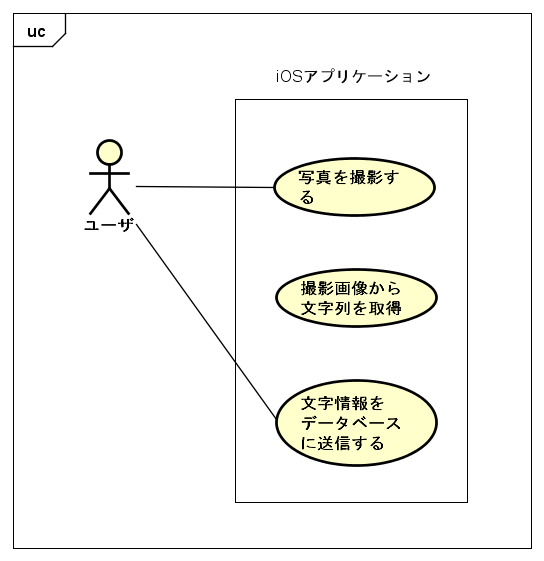
\includegraphics[width=14cm]{fig/usecase_ios.png}
\end{center}
\caption{iOSアプリケーションのユースケース図}
\end{figure}

\subsection{クラス}
\begin{figure}
\begin{center}
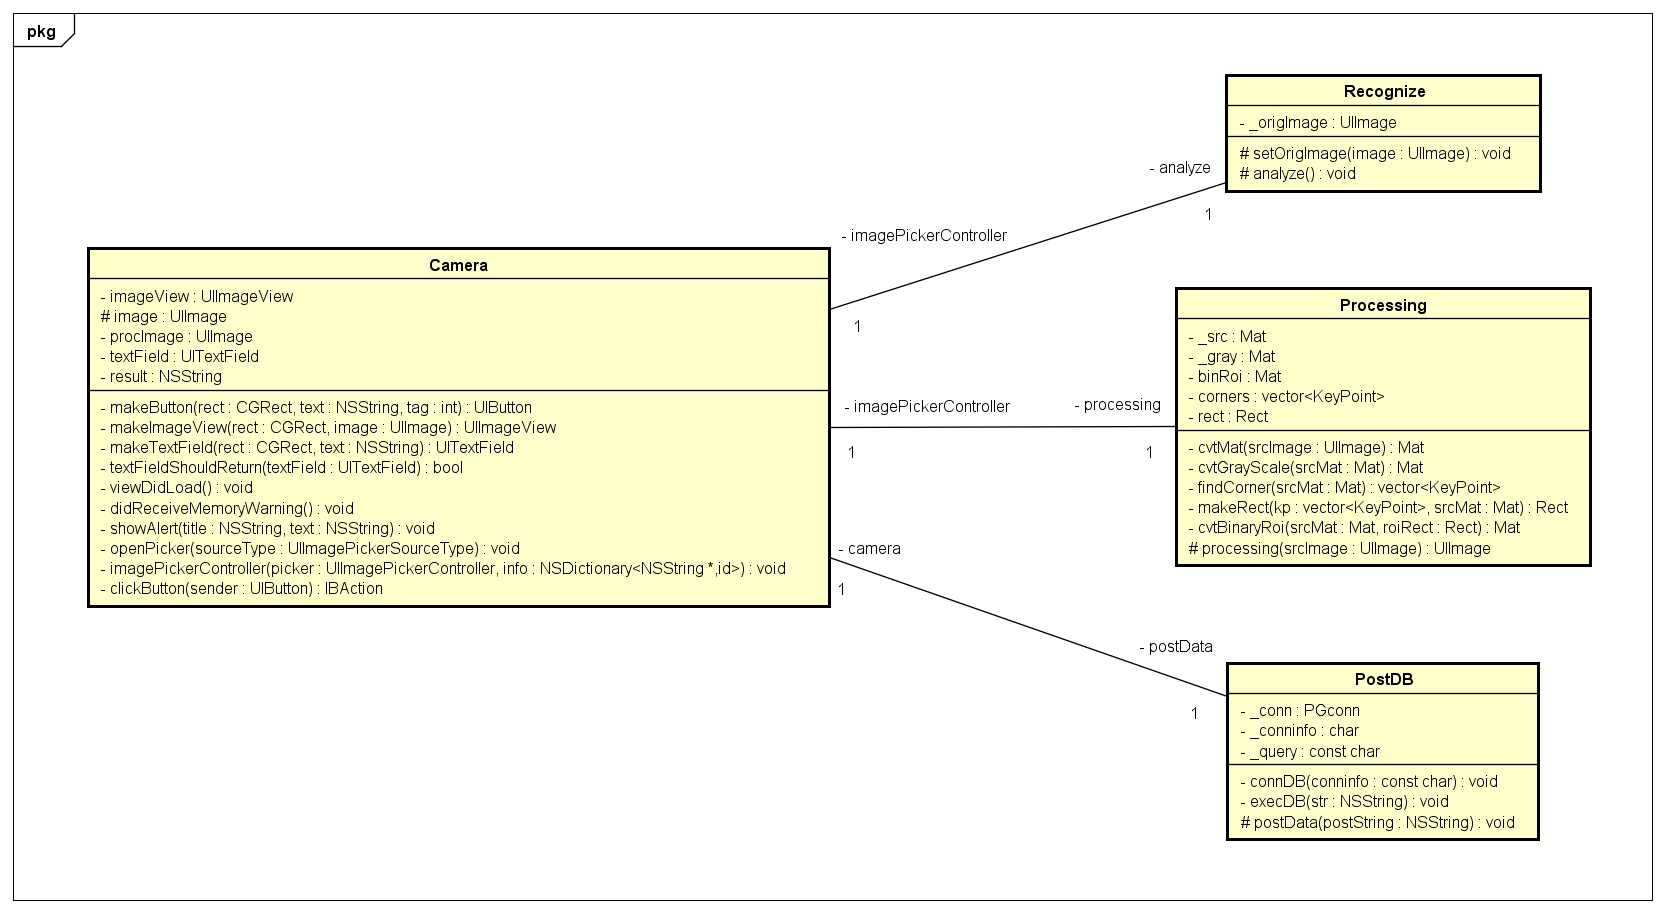
\includegraphics[width=17cm]{fig/class_ios.png}
\end{center}
\caption{iOSアプリケーションのクラス図}
\end{figure}

\subsubsection{(A) Cameraクラス}
Cameraクラスでは, 「iOSアプリケーションのMainViewにボタン等を配置する」, 「iOSデバイスのカメラを起動し, 撮影した画像を保存する」, 「他クラスのメソッドを呼び出す」ことが可能である.

\begin{itemize}
\item 属性

\begin{itemize}
\item imageView:UIImageView

撮影した画像を出力するためのローカル変数.
出力画像のサイズ等を決定する.

\item image:UIImage

撮影した画像を格納するための変数.

\item procImage:UIImage

Processingクラスにて画像処理された画像を格納するための変数.
procImageに格納されている画像を用いて, 光学的文字認識を行う.

\item textField:UITextField

Recognizeにて取得した文字列を表示するテキストボックス.

\item result:NSString

Recognizeにて取得してきた文字列を格納するためのローカル変数.
\end{itemize}

\item 操作

\begin{itemize}
\item makeButton:UIButton

iOSアプリケーションのMainViewにボタンを作成するメソッド.

ボタンを配置する座標, サイズ, ボタンに書かれる文字列, ボタンに付加するタグを指定して呼び出すことで, iOSアプリケーションのMainViewにボタンを作成し配置する.

\begin{itemize}
\item rect:CGRect

ボタンの座標, サイズを決定する変数.

\item text:NSString

ボタンに書かれる文字列を決定する変数.

\item tag:int

ボタンに整数型のタグを付加するための変数.
\end{itemize}

\item makeImageView:UIImageView

iOSアプリケーションのMainViewに画像を表示するためのSubViewを作成するメソッド.

画像を配置する座標, サイズ, 出力する画像を指定して呼び出すことで, iOSアプリケーションのMainViewに画像を出力する.

\begin{itemize}
\item rect:CGRect

画像を出力するSubViewの座標, サイズを指定する変数.

\item image:UIImage

SubViewに出力する画像を指定する変数.
\end{itemize}

\item makeTextField:UITextField

iOSアプリケーションのMainViewにテキストフィールドを作成するメソッド.

テキストフィールドを配置する座標, サイズ, 入力されるテキストを指定して呼び出すことで, iOSアプリケーションのMainViewにテキストフィールドを作成し配置する.

\begin{itemize}
\item rect:CGRect

テキストフィールドを配置する座標, サイズを指定する変数.

\item text:NSString

テキストフィールドに入力する文字列を指定する変数.
\end{itemize}

\item textFieldShouldReturn:BOOL

テキストフィールドにて, キーボードでリターンキーを押した際の挙動を制御するメソッド.

文字列を編集後にリターンキーを押した際に呼び出され, SubViewとして呼びだされているキーボードを引っ込める.

\begin{itemize}
\item textField:UITextField

編集したい文字列が入力されているテキストフィールド.
\end{itemize}

\item viewDidLoad:void

アプリケーションが起動した際に一度だけ読み込まれるメソッド.

変数の初期化やMainViewにボタン等を配置する際に利用する.

\item didReceiveMemoryWarning:void

iOSアプリケーション使用時に, メモリが不足する際に呼び出されるメソッド.

すべてのViewに対して参照を開放する際に利用する.

\item showAlert:void

アラートビューを表示するメソッド.

アラートビューのタイトルと表示するアラートの内容を指定して呼び出すことで, iOSアプリケーションのMainView上にSubViewとしてアラートが表示される.

\begin{itemize}
\item title:NSString

アラートビューのタイトルを指定する変数.

\item text:NSString

アラートビューに表示するテキストを指定する変数.
\end{itemize}

\item openPicker:void

iOSアプリケーションにて, 画像を取得するためのメソッド.

カメラ, フォトアルバム, フォトライブラリから画像を取得する.

このメソッドでは, iOSのカメラ機能にて撮影した画像を取得する際に呼び出す.

\begin{itemize}
\item sourceType:UIImagePickerSourceType

イメージピッカーの属性を決定する変数.
カメラ, フォトアルバム, フォトライブラリのいずれかから選択する.
\end{itemize}

\item imag:PickerController:void

画像取得後に呼び出されるメソッド.

画像を取得した後の処理を行う他クラスのメソッドを呼び出す.

\begin{itemize}
\item picker:UIImagePickerController

画像取得元のイメージピッカーを指定する変数.

\item info:NSDictionary$<$NSString *, id$>$

取得した画像の情報を格納する変数.
\end{itemize}

\item clickButton:IBAction

iOSアプリケーション上のMainViewに配置されているボタンを押下した際に呼び出されるメソッド.

\begin{itemize}
\item sender:UIButton

どのボタンが押下されたのかを決定する変数.
\end{itemize}

\end{itemize}

\end{itemize}

\subsubsection{(B) Processingクラス}
Processingクラスでは, 「撮影画像をOpenCVにて加工可能となるように処理を施す」, 「撮影画像中の文字列が含まれている箇所に注目する」, 「注目している箇所のみで光学的文字認識が施されるように, 撮影画像を加工する」ことが可能である.

\begin{itemize}
\item 属性

\begin{itemize}
\item \_src:Mat

入力画像を指定する変数.

\item \_gray:Mat

グレースケール変換された画像を格納する変数.

\item binRoi:Mat

バイナリスケール変換された画像を格納する変数.

\item corners:vector$<$KeyPoint$>$

検出した特徴点を格納する変数.

\item rect:Rect

特徴点を内包した矩形の座標, サイズ決定する変数.

\end{itemize}

\item 操作

\begin{itemize}
\item cvtMat:Mat

UIImage型の画像をMat型に変換するメソッド.

UIImage型の入力画像を指定して呼び出すことで, OpenCVで処理可能なMat型に変換する.

\begin{itemize}
\item srcImage:UIImage

UIImage型の画像を格納する変数.
\end{itemize}

\item cvtGrayScale:Mat

Mat型画像をグレースケール化するメソッド.

cvtMatにてMat型に変換した入力画像にグレースケール化処理を施す.

\begin{itemize}
\item srcMat:Mat

3チャネルの入力カラー画像を格納する変数.
\end{itemize}

\item findCorner:vector$<$KeyPoint$>$

グレースケール画像から特徴点を検出するメソッド.

cvtGrayScaleにてグレースケール処理を施した画像を指定することで, その画像中から特徴点を検出する.

\begin{itemize}
\item srcMat:Mat

グレースケール画像を格納する変数.
\end{itemize}

\item makeRect:Rect

特徴点を内包する矩形の座標, サイズを決定するメソッド.

特徴点の集合を指定することで, 特徴点の多い部分に注目するための矩形を設定する.

\begin{itemize}
\item kp:vector$<$KeyPoint$>$

特徴点の集合を格納する変数.

\item srcMat:Mat

グレースケール画像を格納するための変数.
\end{itemize}

\item cvtBinaryRoi:Mat

Mat型カラー画像をバイナリ画像へ変換するメソッド.

makeRectにて設定した矩形を指定することで, 注目している範囲をバイナリ画像化する.

\begin{itemize}
\item srcMat:Mat

3チャネルの入力カラー画像を格納する変数.

\item roiRect:Rect

注目する矩形範囲を決定する変数.
\end{itemize}

\item processing

Processingクラスのメソッドをコントロールするメソッド.

\begin{itemize}
\item srcImage:UIImage

CameraクラスのopenPickerControllerメソッドにて取得した撮影画像を格納する変数.
\end{itemize}

\end{itemize}

\end{itemize}

\subsubsection{(C) Recognizeクラス}
Recognizeクラスでは, 「光学的文字認識を実行する」, 「取得した文字列をCameraクラスに渡す」ことが可能である.

\begin{itemize}
\item 属性

\begin{itemize}
\item \_origImage:UIImage

光学的文字認識を実行する画像を格納するための変数.
\end{itemize}

\item 操作

\begin{itemize}
\item setOrigImage:void

光学的文字認識を実行する画像を取得するためのメソッド.

Processingクラスのprocessingメソッドにて処理の施された画像を受け取り, \_origImageに格納する.
\begin{itemize}
\item image:UIImage

光学的文字認識を施す画像を指定する変数.
\end{itemize}

\item analyze:void

Tesseract-OCRによる光学的文字認識を実行するメソッド.
\end{itemize}

\end{itemize}

\subsubsection{(D) PostDBクラス}
\begin{itemize}
\item 属性

\begin{itemize}
\item \_conn:PGconn

PostgreSQLデータベースとの接続状態を格納する構造体.

\item \_conninfo:const char

PostgreSQLデータベースの接続する際に必要となる情報を格納する変数.

\item \_query:char

接続したPostgreSQLにて実行するクエリを決定する変数.
\end{itemize}

\item 操作

\begin{itemize}
\item connDB:void

WebアプリケーションのPostgreSQLに接続するメソッド.
\begin{itemize}
\item conninfo:const char

PostgreSQLへの接続状態を保存する変数.
\end{itemize}

\item execDB:void

WebアプリケーションのPostgreSQLデータベースへクエリを発行し, データベースへデータを追加する.
\begin{itemize}
\item str:NSString

PostgreSQLデータベースへ送信する文字列を決定する変数.
\end{itemize}

\item postData:void

PostDBクラスのメソッドをコントロールするメソッド.
\begin{itemize}
\item postString:NSString

WebアプリケーションのPostgreSQLデータベースへ送信する文字列を決定する変数.
\end{itemize}

\end{itemize}

\end{itemize}

\section{Webアプリケーション}
Webアプリケーションを作成するにあたり, 以下の言語とライブラリ, サービスを利用した.(表3.2参照.)

\begin{table}
\begin{center}
\begin{tabular}{|l|l|} \hline
rbenv & \\ \hline
Ruby & \\ \hline
RubyGems & \\ \hline
Ruby on Rails & \\ \hline
PostgreSQL & \\ \hline
Heroku & \\ \hline
\end{tabular}
\end{center}
\caption{Webアプリケーション作成時に利用した環境のバージョン一覧}
\end{table}

\subsection{要件定義}
Webアプリケーションには, 以下の機能を実装する.

\begin{itemize}
\item データベースにて, iOSアプリケーションから送信された文字列を送信された日時/時刻とともに管理する.

\item 集積したデータを文字列, 日付にて検索する.
\end{itemize}

これらの要件を, UMLを用いて分析する.

\subsection{ユースケース}
ユーザはiOSアプリケーションから送信された全データを閲覧することができ, 文字列, 送信した日付で検索することができる.

\begin{figure}
\begin{center}
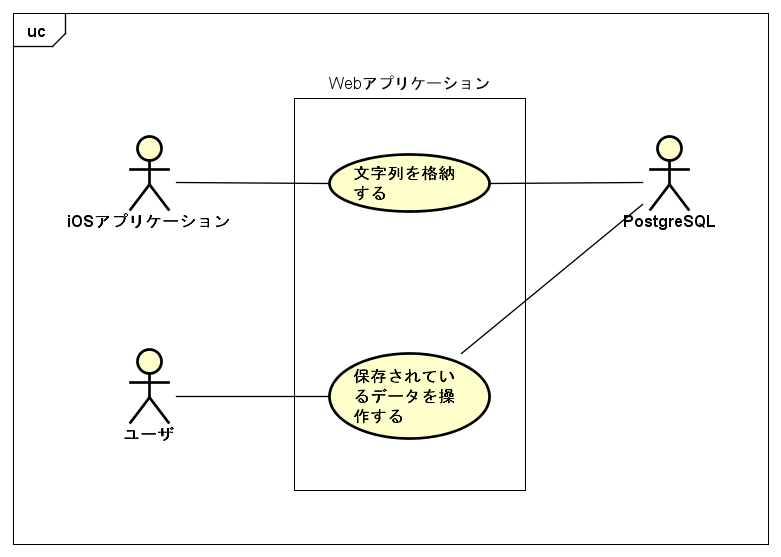
\includegraphics[width=10cm]{fig/usecase_web.png}
\end{center}
\caption{Webアプリケーションのユースケース図}
\end{figure}

\subsection{クラス}

\begin{figure}
\begin{center}
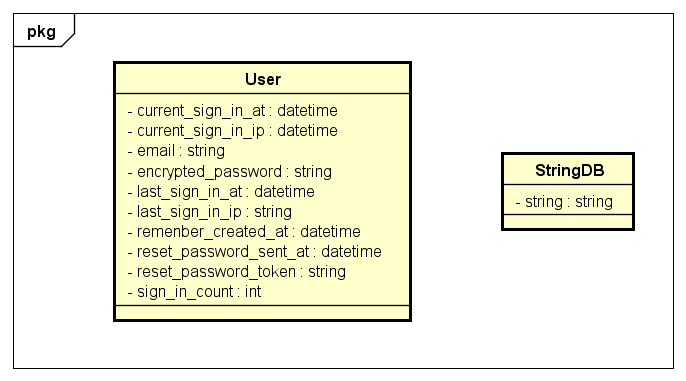
\includegraphics[width=13cm]{fig/class_web.png}
\end{center}
\caption{Webアプリケーションのクラス図}
\end{figure}

\subsubsection{(A) Userクラス}
\begin{itemize}
\item 属性

\begin{itemize}
\item current\_sign\_in\_at:datetime

Webアプリケーションにユーザ登録したユーザがサインインした時刻を記録するカラム.

\item current\_sign\_in\_ip:datetime

ユーザがサインインした際のリモートIPを記録するカラム.

\item email:string

ユーザのサインイン時に利用するEメールアドレスを記録するカラム.

\item last\_sign\_in\_at:datetime

ユーザが最終サインインした時刻を記録するカラム.

\item last\_sign\_in\_ip:datetime

ユーザが最終サインインした際のリモートIPを記録するカラム.

\item remenber\_created\_at:datetime

ユーザ登録した時刻を記録するカラム.

\item reset\_password\_sent\_at:datetime

パスワードをリセットする操作を行った際の時刻を記録するカラム.

\item reset\_password\_token:string

パスワードをリセットする操作を行った際に設定した新しいパスワードを記録するカラム.

\item sign\_in\_count:int

ユーザがサインインした回数を記録するカラム.
\end{itemize}

\end{itemize}

\subsubsection{(B) StringDBクラス}
\begin{itemize}
\item 属性

\begin{itemize}
\item string:string

光学的文字認識にて取得した文字列を記録するカラム.
\end{itemize}

\end{itemize}



\chapter{本研究の利用例, 利用アイデア}
\label{chap:utilization}

本研究では, 「iOSのポータビリティの高さ」と「沖縄県の観光産業」に注目し, 観光地の文字情報をデータベースに集積することを行った.

しかし, 本研究は上記の目的のみにとどまらず, iOSデバイスのポータビリティを活かし, 様々な分野に派生することが可能であると考える.

\section{利用アイデア1:緊急車両や警察車両への住所通達システム}
\subsection{背景と目的}
本研究にて構築したシステムは, スマートデバイスで撮影した画像から文字列を取得し, Webアプリケーションのデータベースに送信する, というものである.

ここでは, 画像に“GPSによる位置情報”を付与する.

SNSが急速に普及して以降, 事件や事故が起きた際に, その現場周辺にいる人々がその様子を撮影し, SNSにその時の状況をアップロードする, ということが行われるようになっている.
ここでは, その“画像による状況把握の容易さ”と, “スマートデバイスにてGPSの位置情報が利用可能である”ことに注目する.

\subsection{システムの要件定義}
ユーザが現場周辺でスマートデバイスを用いて画像を撮影する.
その画像にGPSの位置情報とどの緊急車両(救急, 消防, 警察)が必要であるかの情報を付与し, Webアプリケーションに送信する.

受信したWebアプリケーションは, それらの情報を受け取ると各緊急機関に現場画像と位置情報, どの緊急車両を向かわせるか要請する.

そして, 緊急車両は指定された車両でGPSによる現場の位置情報を元に, 現場に向かう.

\subsection{このシステムを利用することで解決する問題}
このシステムを利用することで解決する問題は,
\begin{itemize}
\item 緊急車両を呼ぶ際に, 現場の住所がすぐに分からない

現場の住所を電話口で職員に伝える際, 通報者の近くに現住所を示すものがない場合, 正確な住所を伝えることが困難となることも考えられる.

このシステムでは, スマートデバイスから取得したGPSの位置情報をWebアプリケーションに送信するため, 住所が不明な場所においても, 正確な現場の位置を伝えることが可能となる.

\item 偽情報による緊急車両の出動

通報による緊急車両の出動は, 故意な偽情報によって行われることがある.
それらの悪意ある行動による緊急車両の不必要な出動は, 真に必要な現場への出動が遅延する可能性を生む.

このシステムでは, スマートデバイスのポータビリティと情報発信力を活用しており, 大規模な事件, 事故の場合は複数人が通報システムを利用することが考えられるため, 偽情報による緊急車両の出動を抑制することが可能だと推測できる.
\end{itemize}



\chapter{今後の展開}
\label{chap:problem}



\def\line{-\hspace*{-.7zw}-}

\begin{thebibliography}{99}

\bibitem{1}
\url{http://www.soumu.go.jp/johotsusintokei/whitepaper/ja/h25/html/nc243110.html}
\bibitem{2}
\url{https://ja.wikipedia.org/wiki/Objective-C}
\bibitem{3}
\url{https://developer.apple.com/jp/documentation/ObjC.pdf}
\bibitem{4}
\url{https://developer.apple.com/support/xcode/jp/}
\bibitem{5}
\url{http://www.buildinsider.net/small/opencv/001}
\bibitem{6}
\url{http://www.apple.com/jp/osx/continuity/}
\bibitem{7}
\url{http://allabout.co.jp/gm/gc/3588/}
\bibitem{8}
\url{http://news.mynavi.jp/news/2015/08/06/144/}
\bibitem{9}
\url{http://windows.microsoft.com/ja-jp/windows/history#T1=era0}
\bibitem{10}
\url{https://en.wikipedia.org/wiki/List_of_Microsoft_Windows_versions}
\bibitem{11}
\url{http://marketshare.hitslink.com/operating-system-market-share.aspx?qprid=8&qpcustomd=1}
\bibitem{12}
\url{https://github.com/tesseract-ocr/tesseract/blob/master/README.md}
\bibitem{13}
\url{https://ja.wikipedia.org/wiki/Model_View_Controller}
\bibitem{14}
\url{http://www.rubylife.jp/rails/ini/index7.html}
\bibitem{15}
\url{http://codezine.jp/article/detail/8051}
\bibitem{16}
\url{http://e-words.jp/w/RDBMS.html}
\bibitem{17}
\url{https://en.wikipedia.org/wiki/CentOS}

\end{thebibliography}

\chapter*{謝辞}
\thispagestyle{empty}

\hspace{1zw}本研究の遂行、また本論文作成にあたり、御多忙にもかかわらず終始懇切なる御指導と御教授を賜りました谷口祐治准教授に深く感謝致します。

また、一年間共に研究を行い、温かな気遣いと励ましをもって支えてくれた学習環境システム研究室の山本耀悟君、大濱ゆめさん、ならびに琉球大学工学部情報工学科インターネットシステム研究室の皆様に感謝致します。

最後に、有意義な時間を共に過ごした情報工学科の学友、ならびに物心両面で支えてくれた両親に深く感謝致します。

\begin{flushright}
\today \\ 長倉貴洋
\end{flushright}

\end{document}